\section{\textsf{Simulation}}
    The simulation has be created using the CST software in order to implement a configuration such as shown in \cite{zhang_design_2023}.

    \subsection{\textsf{CST Implementation}}
        The vertical layout implemented in CST consists of a three layer structure:
        \begin{itemize}
            \item Dielectric substrate
            \item Air
            \item Metal Backplate
        \end{itemize}

        The dielectric substrate will also embody a metallic component made of the same material as the metal backplate; copper
        (5.96 \mu $10^7$ S/m).

        At first I'll place the substrate without the resonance layer:  
        \begin{figure}[h]
            \centering
            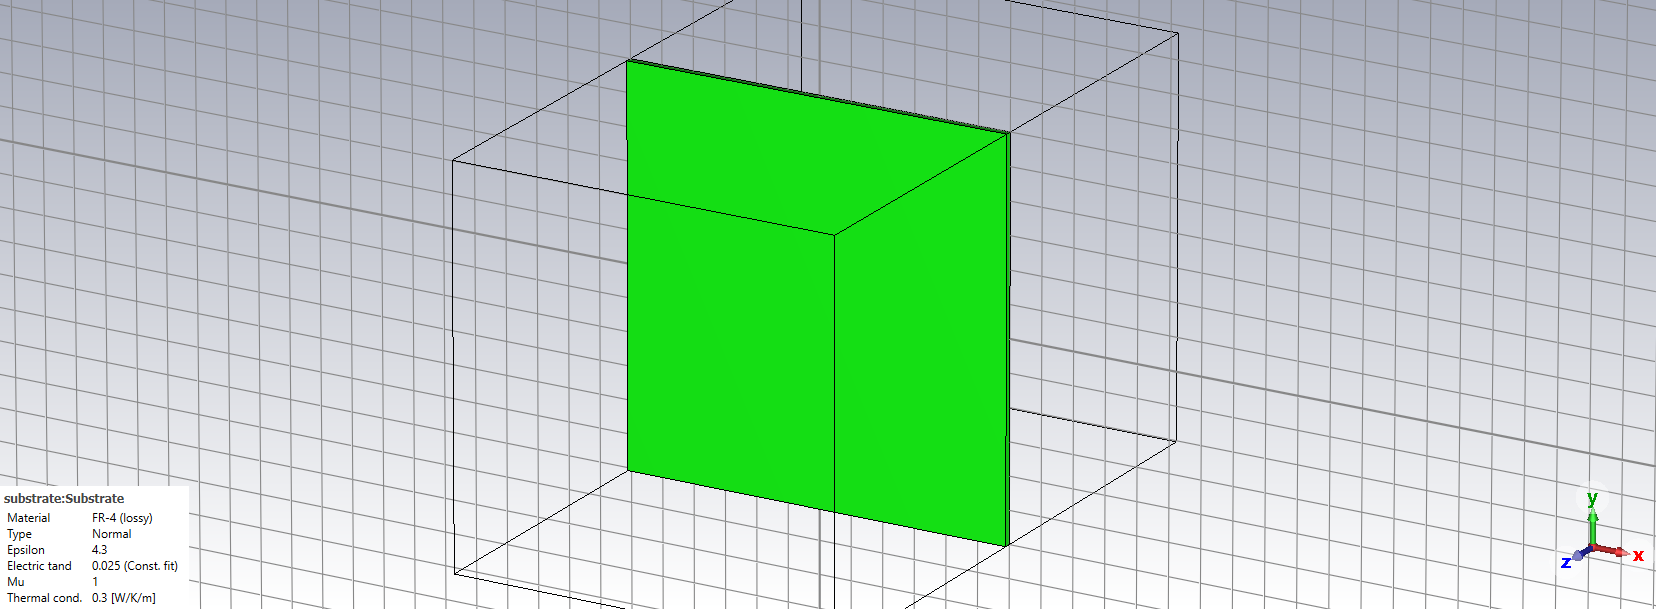
\includegraphics[width=\textwidth]{substrate.png}
            \caption{FR-4 Dielectric Substrate}
            \label{img:substrate}
        \end{figure}

        Later I'll place the metal resonance layer as well but there are a number of possible candidates
        I think of trying to simulate whereas the vertical layout is pretty much fixed.

        I'll place the two other layers below Z=0, turn on the orthographic side
        view to remove shadows and voila: 
        \begin{figure}[b]
            \centering
            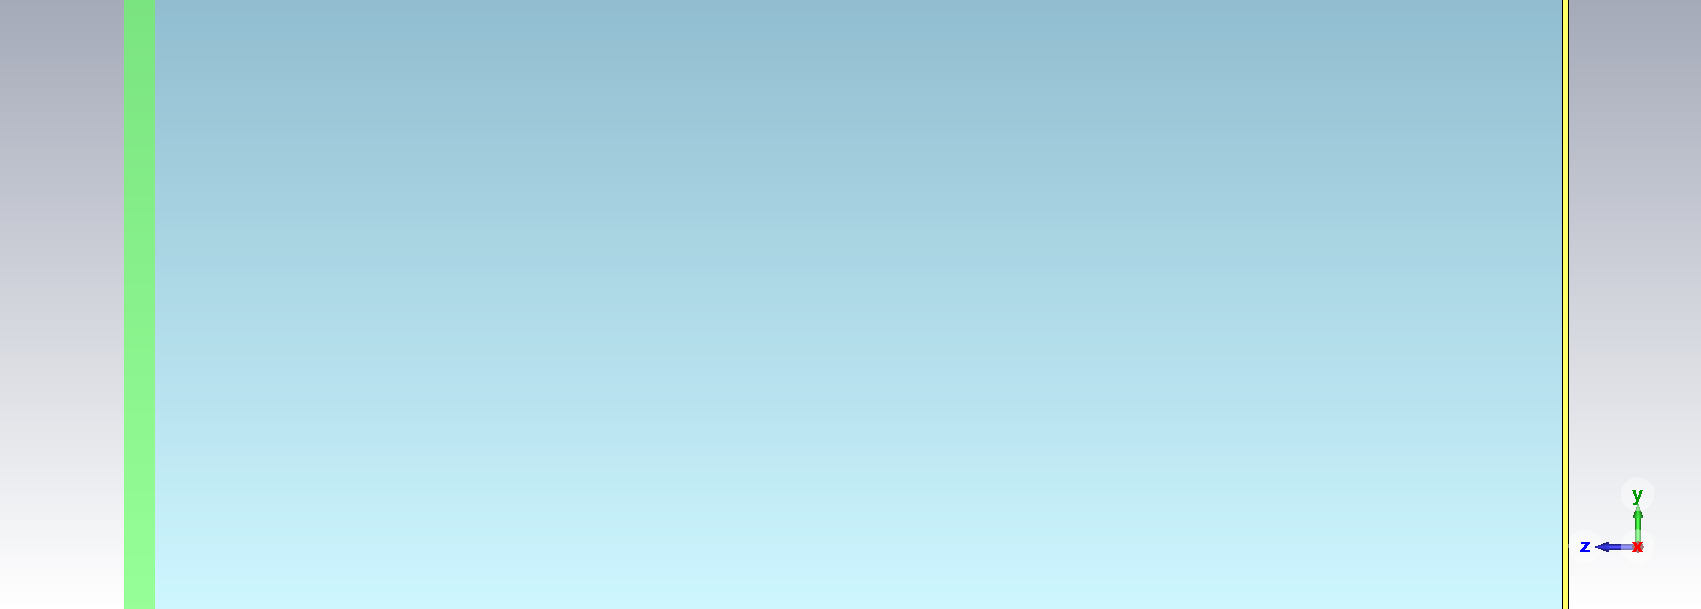
\includegraphics[width=\textwidth]{verticaLayout.png}
            \caption{Vertical Layout Orthographic View}
            \label{img:verticaLayout}
        \end{figure}
        I think it really gives a sense of scale as the air layer truly shadows the other two.

        Now its time to add the ring that is of the same material and thickness as the backplate and lies
        on top of the dielectric substrate. 
        \begin{figure}[b]
            \centering
            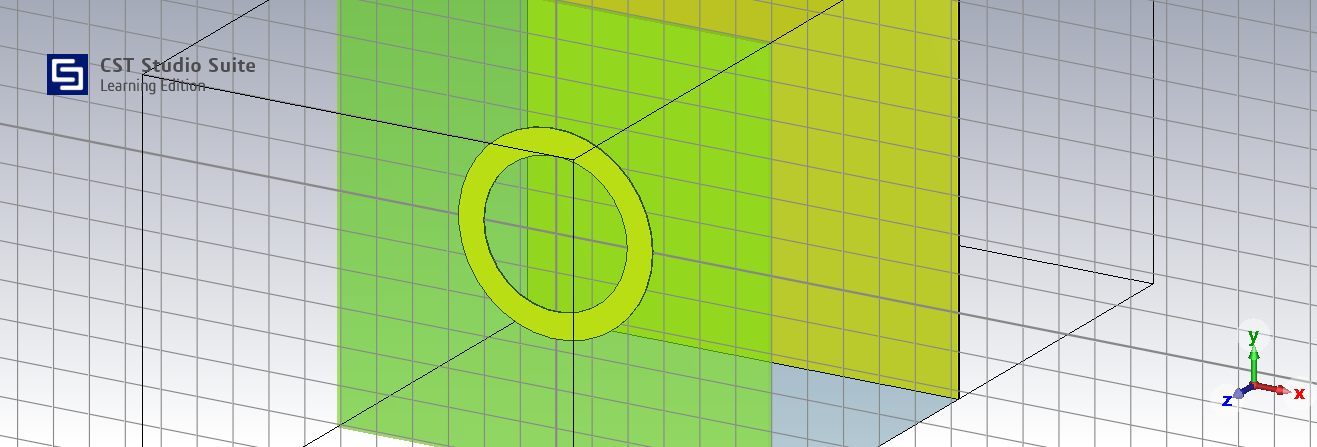
\includegraphics[width=\textwidth]{ring.png}
            \caption{Ring Resonator}
            \label{img:ring}
        \end{figure}

        Then I will move the substrate, air and backplate layers all below Z=0 just ti make is easier
        with designing the arrows. For this I make the assumption that both the arrow body and point are
        a=0.5mm of width. 
        \begin{figure}[h]
            \centering
            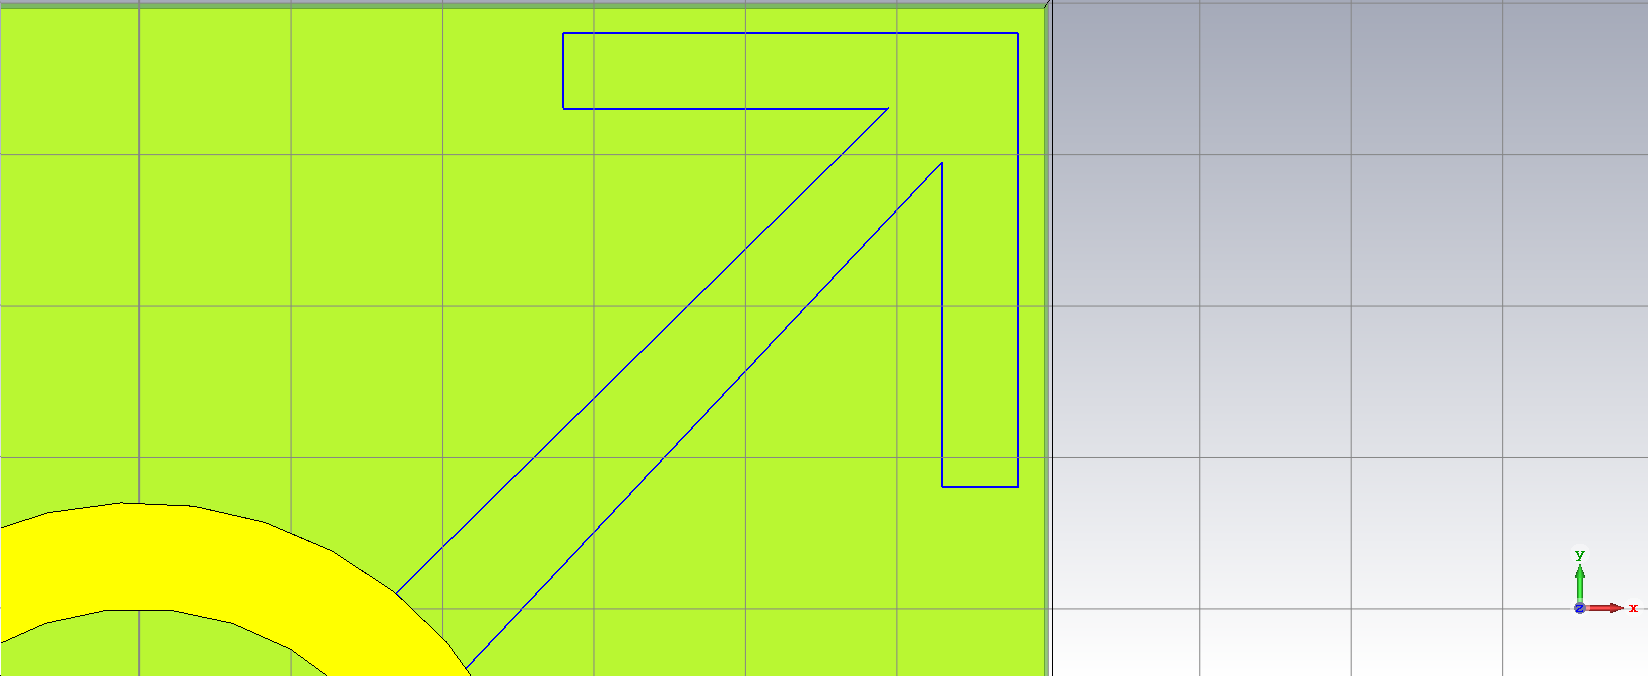
\includegraphics[width=\textwidth]{parallel.png}
            \caption{Initial Arrow Base}
            \label{img:parallel}
        \end{figure}
        In order to accurately place all the curve points that define the arrow some basic calculations
        shall be made. The two points of the arrow base lie exactly on the arc of the ring and are 
        equidistant from curve y=x so the in order to find their cartesian coordinates the following
        system shall be solved. 

        \begin{lstlisting}[frame=single, numbers=left, style=Matlab-Pyglike]
            syms x1 x2

            eq1 = 2*(x1 - x2)^2 == .5^2;
            eq2 = sqrt(x2^2 + x1^2) == 2.7;

            sol = solve([eq1, eq2], [x1 x2]);
            disp([sol.x1 sol.x2]);  
        \end{lstlisting}
        
        \begin{equation}
            \label{eq:xysys}
            \displaystyle \begin{array}{l} 
                \left(\begin{array}{cc} 
                    \sigma_3 -\frac{2916\,\sigma_1 }{1433} & -\sigma_1 \\
                    \sigma_4 -\frac{2916\,\sigma_2 }{1433} & -\sigma_2 \\
                    \frac{2916\,\sigma_1 }{1433}-\sigma_3  & \sigma_1 \\
                    \frac{2916\,\sigma_2 }{1433}-\sigma_4  & \sigma_2  
                \end{array}\right)\\
                \mathrm{}\\
                \textrm{where}\\
                \mathrm{}\\
                \;\;\sigma_1 =\sqrt{\frac{729}{200}-\frac{7\,\sqrt{59}}{80}}\\
                \mathrm{}\\
                \;\;\sigma_2 =\sqrt{\frac{7\,\sqrt{59}}{80}+\frac{729}{200}}\\
                \mathrm{}\\
                \;\;\sigma_3 =\frac{400\,{{\left(\frac{729}{200}-\frac{7\,\sqrt{59}}{80}\right)}}^{3/2} }{1433}\\
                \mathrm{}\\
                \;\;\sigma_4 =\frac{400\,{{\left(\frac{7\,\sqrt{59}}{80}+\frac{729}{200}\right)}}^{3/2} }{1433}
            \end{array}
        \end{equation}

        Which results in two points/quadrant so picking out the two points of the 1st quadrant and 
        inserting them to CST the arrow body is parallel again 
        \begin{figure}[h]
            \centering
            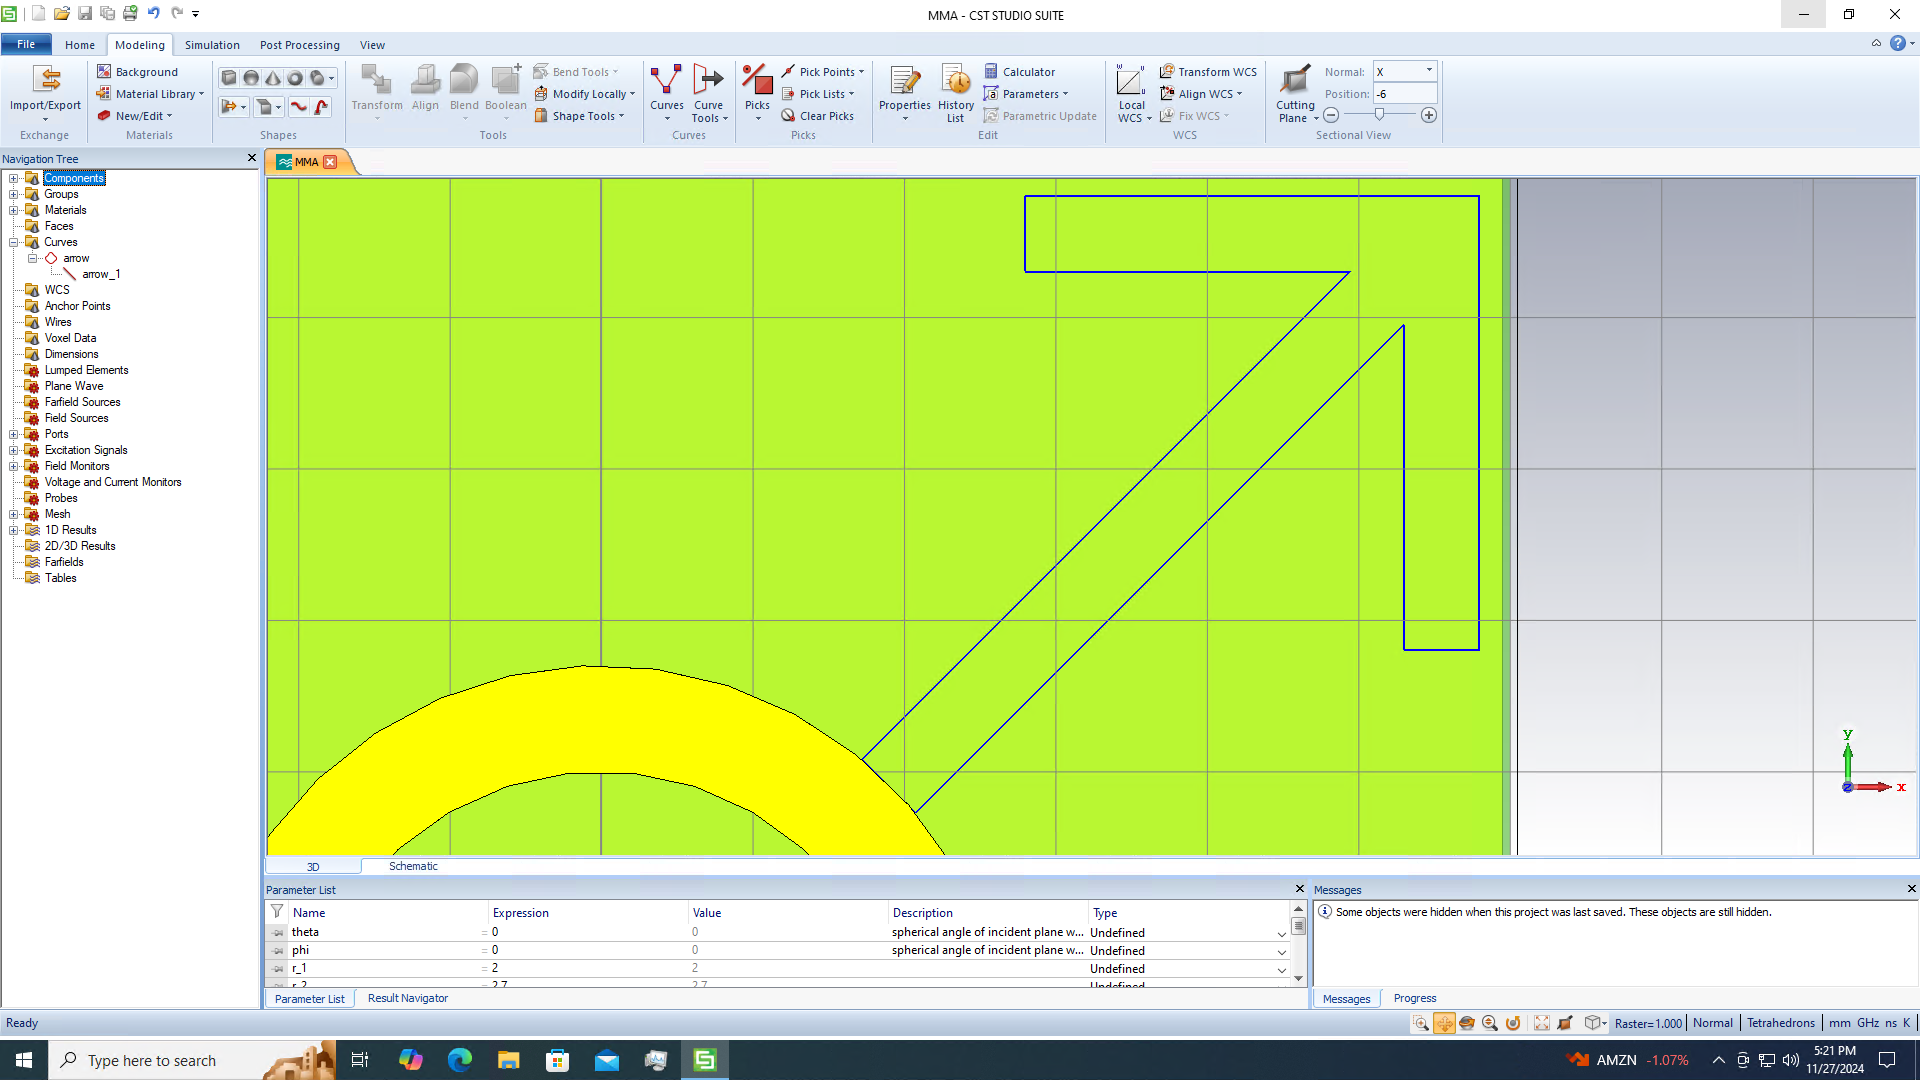
\includegraphics[width=\textwidth]{corretArrowBase.png}
            \caption{Correct Arrow Base}
            \label{img:corretArrowBase}
        \end{figure}

        Then the arrow is mirrored against the X, the Y and the XY planes in order to reach all four 
        sides of the cell, then the face is covered with copper and a height of d=0.035mm is also 
        attributed, which is why it was important to move all other layers below Z=0. 
        \begin{figure}[h]
            \centering
            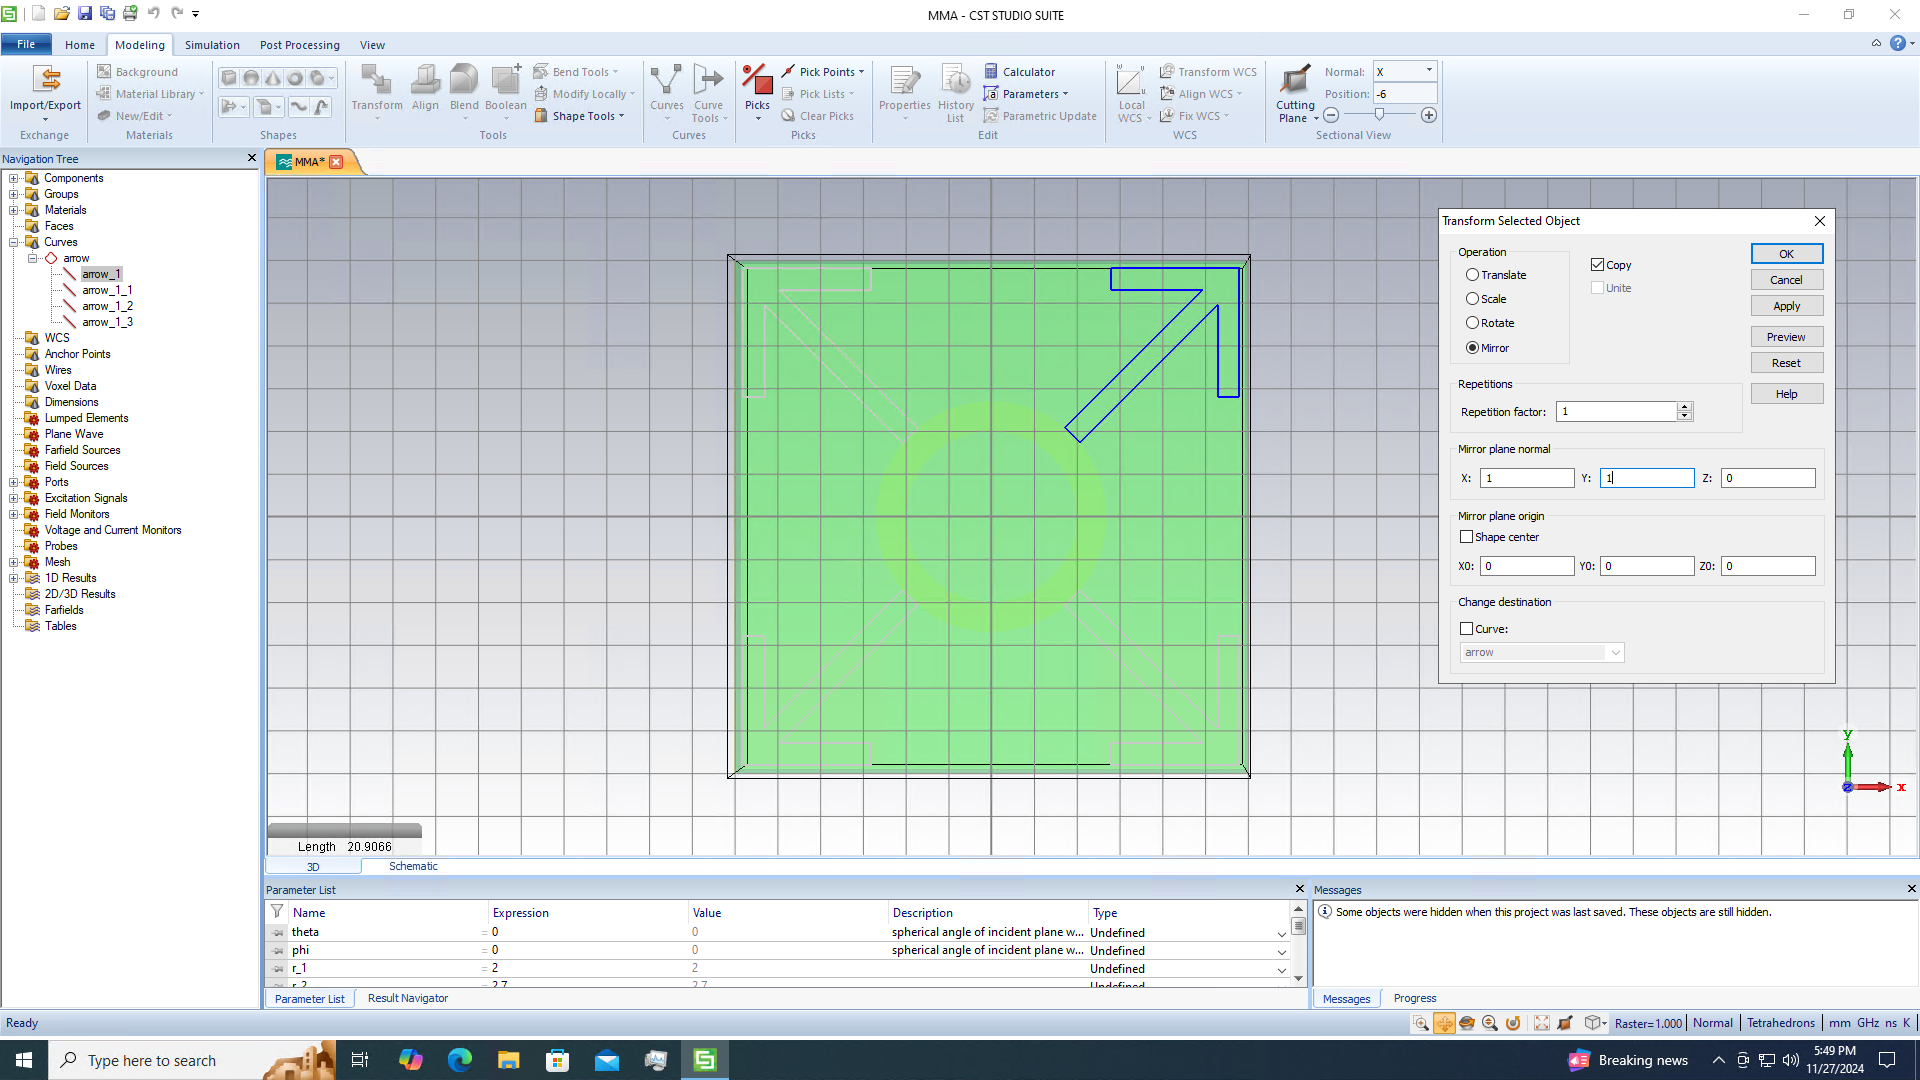
\includegraphics[width=.4\textwidth]{mirroredArrows.png}\hfil
            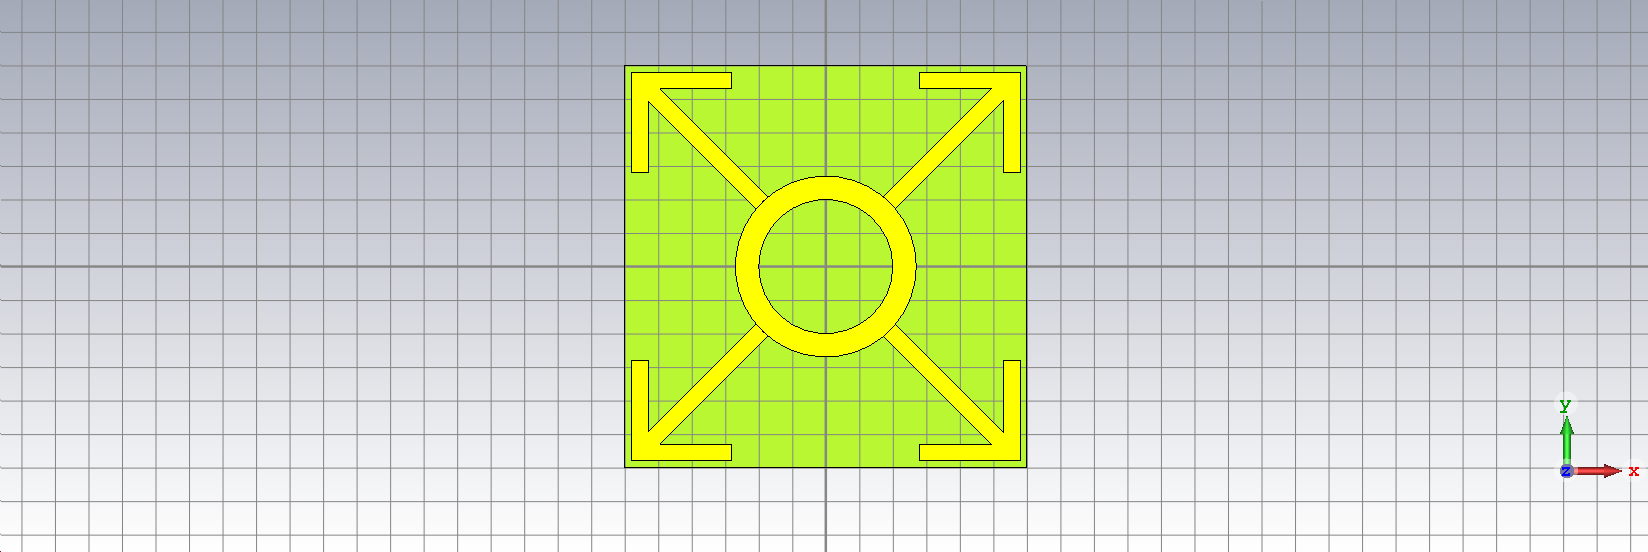
\includegraphics[width=.4\textwidth]{RingAndArrows.png}
            \caption{Mirroring Arrow and Cover}
            \label{img:mirrorAndCover}
        \end{figure}
        

        Now I'll try and perform a simulation using the frequency solver in CST just to get an idea 
        how the component behaves, the boundaries will be periodic along the XY plate and I will add
        absorbing conditions along the Z axis.

        For reference the mesh with only the ring element on the surface ends up such as: 
        
        \begin{figure}[h]
            \centering
            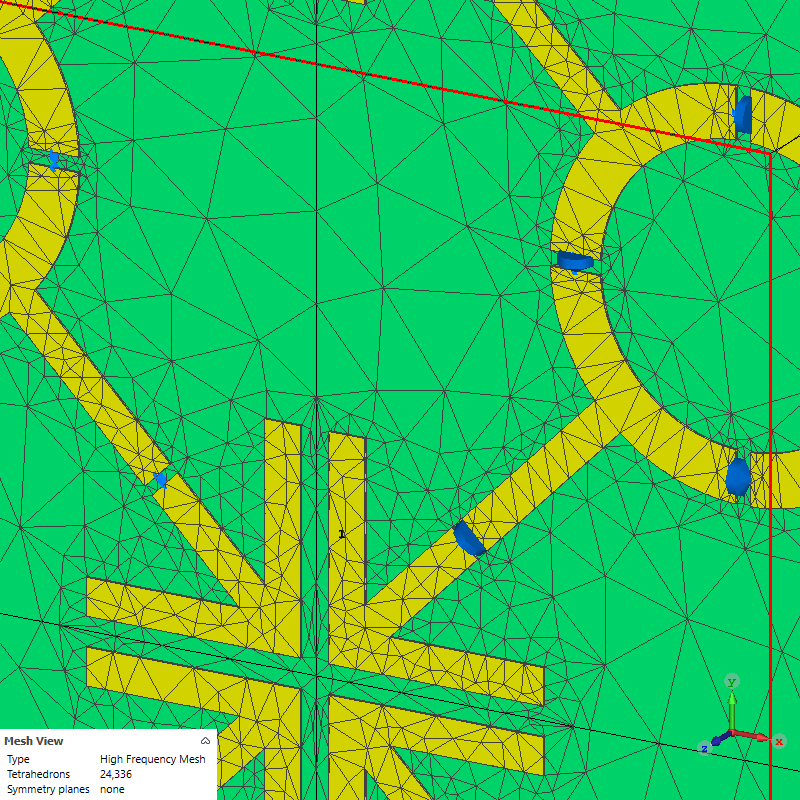
\includegraphics[width=\textwidth]{mesh.png}
            \caption{Ring Mesh for reference}
            \label{img:ringMesh}
        \end{figure}

        Now the Mesh that ends up including the arrows is as such:
        \begin{figure}[h]
            \centering
            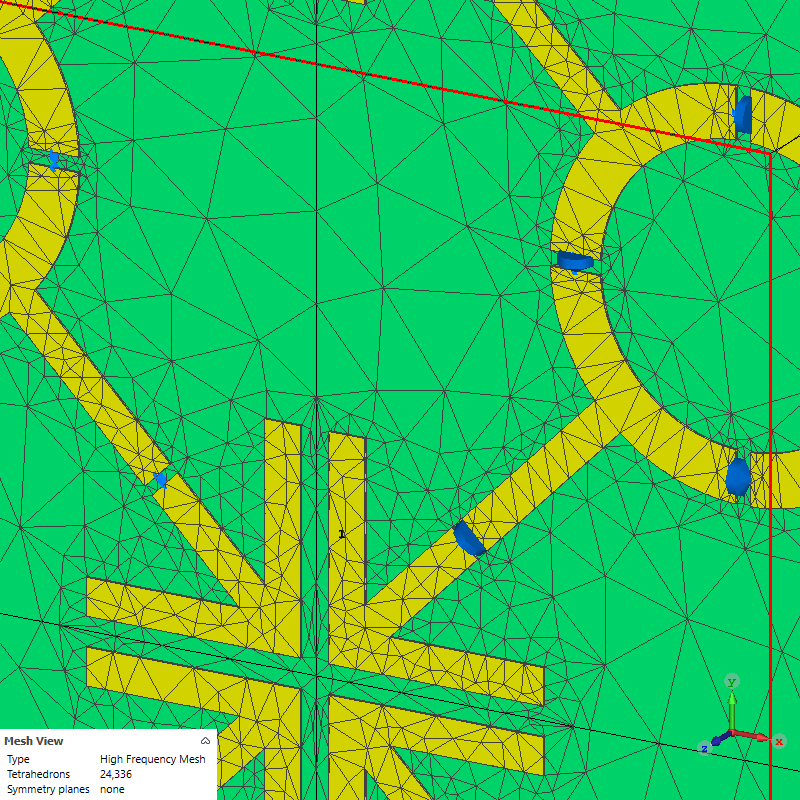
\includegraphics[width=\textwidth]{mesh.png}
            \caption{Ring Mesh for reference}
            \label{img:RingAndArrowMesh}
        \end{figure}

        Taking a look in the E-Field after the simulation it behaves as such:
        \begin{figure}[h]
            \centering
            \animategraphics[width=\textwidth, autoplay, loop, controls]
            {8}{gif/MMA_UnitCell_E_27e2MHz_Zmax1-}{0}{71}
            \caption{UnitCell E field 2.7GHz Zmax(1)}
            \label{fig:UnitCell_E_27e2MHz_Zmax1}
        \end{figure}

    \subsection{\textsf{Alternative Modeling Methods}}
        In order to simulate the absorber there are also a few other ways to go about it:
        \begin{itemize}
            \item Transmission Line equivalent
            \item Electrical circuit equivalent
            \item Mathematical modeling \& code (MATLAB)
        \end{itemize}

        So at first I start by designing a basic layout in CST..